\documentclass{beamer}
\usepackage{graphicx} % Required for inserting images

\usetheme{Berkeley}
\usecolortheme{beaver}

\usepackage[slovene]{babel}




\title{Napredna računalniška orodja - 1. domača naloga}
\subtitle{MATLAB, GitHub in Beamer }
\author{Jure Zupančič }
\date{Oktober 2023}

\logo{

\includegraphics[width=1.54cm]{logo.png}
}

\begin{document}

\maketitle

\begin{frame}{Kazalo}
    \tableofcontents[]
\end{frame}

\section{Uvod}

\begin{frame}{Uvod}
    Pri predmetu Napredna računalniška orodja nam je bila podana prva domača naloga, v kateri smo morali izkazati pridobljeno znanje o uporabi orodij MATLAB, Beamer (LaTeX) in GitHub.

\end{frame}


\section{MATLAB}
\begin{frame}{MATLAB 1}
    V MATLABU smo morali z uporabo metode Monte Carlo določiti približek števila $\pi$. To smo storili tako, da smo ustvarili poljubno število točk, katerih x in y koordinate so bile iz intervala $[-0,5 ; 0,5]$. Prikazane so na sliki \ref{fig:enter-label}.

    \pause
    
    \begin{figure}
        \centering
        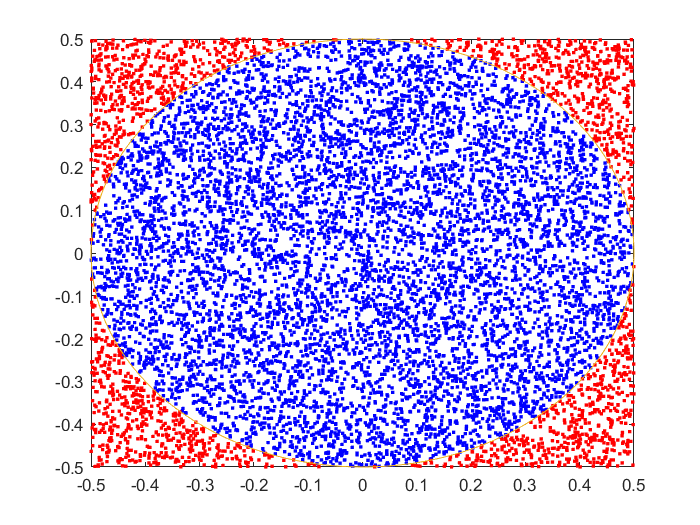
\includegraphics[width=5cm]{točke.png}
        \caption{Točke s katerimi določimo približek števila $\pi$.}
        \label{fig:enter-label}
    \end{figure}
\end{frame}

\begin{frame}{MATLAB 2}
    
    Točke smo nato ločili glede na to ali so ležale znotraj kroga z radijem $r=0,5$ ali zunaj nje.
    S funkcijo smo primerjali število točk zunaj in znotraj kroga in ta podlagi tega določili približek števila $\pi$.
\end{frame}

\section{GitHub}
\begin{frame}{GitHub}
    MATLAB kodo, ki smo jo ustvarili za izračun števila $\pi$ smo nato morali naložiti na naš GitHub repozitorij, ki tudi služi kot sredstvo
    za oddajo domače naloge.
    Naloženo kodo je moral eden izmed naših kolegov dopolniti in sicer opremiti prikaz točk z ustrezno legendo.
\end{frame}


\section{Beamer}
\begin{frame}{Beamer}
    Nazadnje pa smo morali tudi pripraviti predstavitev, ki opisuje opravljeno delo in vsebuje določene zahteve, kot so na primer kazalo, logotip FS in vsaj eno sliko. Predstavitev; tex datoteko, končen pdf in vse uporabljene slike pa smo morali prav tako oddati na naš GitHub repozitorij.
\end{frame}
\end{document}
